\documentclass[11pt]{article}
\usepackage[utf8]{inputenc}
\usepackage[T1]{fontenc} % uses T1 fonts (better quality)
\usepackage{lmodern} % uses Latin Modern fonts
\usepackage[margin=1in]{geometry}
\usepackage[dvipsnames]{xcolor}
\usepackage{ragged2e}
\renewcommand{\baselinestretch}{1.15}
\usepackage{tikz}
\usetikzlibrary{automata,scopes,shapes,matrix,arrows,decorations.pathmorphing}
\tikzset{>={stealth}}
\usepackage{mathtools}
\usepackage{bm}
\usepackage{graphicx}
\usepackage[makeroom]{cancel}
\definecolor{OuterBlue}{HTML}{1370AA}
\definecolor{InnerBlue}{HTML}{9BC4DD}
\usepackage{pdfpages}

\begin{document}
 	\begin{center}
 	\LARGE{ECE 345 / ME 380: Introduction to Control Systems\\Problem Set \#2}\\[1.5em]
 	\large David Kirby\\[1.5em]
 	\large \textbf{Due Thursday, September 17, 2020 at 3:30pm}\\[2.5em]
 	\end{center}

\begin{enumerate}
    \item (+10 points) Consider the system described by
    \begin{align}
        G(s)=\frac{2(s+2)}{s(s+ 4)(s+ 10)}
    \end{align}
    \begin{enumerate}
        \item Find the poles and the zeros of \(G(s)\).
        \begin{align*}
            \text{poles: }s&=0,-4,-10\\
            \text{zeros: }s&=-2
        \end{align*}
        \item Put the transfer function \(G(s)\) in proper form, with one polynomial in the numerator and one polynomial in the denominator.
        \begin{align*}
            G(s)=\frac{2s+4}{s^3+14s^2+40s}
        \end{align*}
        \item Find the characteristic equation of \(G(s)\).
        \begin{align*}
            \Delta(s)=s^3+14s^2+40s=0
        \end{align*}
    \end{enumerate}
    \item (+10 points) The longitudinal dynamics of a vertical take-off and landing aircraft that is hovering are described by:
    \begin{align}
        \dot{x}\quad&=\quad
            \begin{bmatrix*}[r]
            &0 &&1 &&0&\\
            &0 &&0 &&1&\\
            &0 &&-5 &&-2&
            \end{bmatrix*}
            x+
            \begin{bmatrix*}
            &0 &\\
            &0 &\\
            &10&
            \end{bmatrix*}
            u\\[0.75em]\notag
        y\quad&=\quad
        \begin{bmatrix}
            &1 & 0 & 0&\\
        \end{bmatrix}
        x
    \end{align}
    \begin{enumerate}
        \item Find the characteristic equation of this system.
        \begin{align*}
            \Delta(s)&=|sI-A|\\
            &=
            \det \begin{bmatrix*}[r]
                &s &&-1 &&0&\\
                &0 &&s &&-1&\\
                &0 &&5 &&s+2&
            \end{bmatrix*}\\
            &=s^3+2s^2+5s
        \end{align*}
        \item Where are the poles of the system located?
        \begin{align*}
            \text{Eigenvalues}(A)&=0,-1\pm 2i
        \end{align*}
    \end{enumerate}
    \item (+10 points) State-space representations are not unique. A single system can be represented in several possible ways. Consider the following two systems:
    \begin{align*}
        \text{System 1:}\quad
        \begin{cases}
            \begin{bmatrix*}[r]
                &\dot{x_1}&\\
                &\dot{x_2}&
            \end{bmatrix*}
            &=\quad
            \begin{bmatrix*}[r]
                &-3 & 0&\\
                &0 & -2&
            \end{bmatrix*}
            \begin{bmatrix*}[r]
                &x_1&\\
                &x_2&
            \end{bmatrix*}+
            \begin{bmatrix*}[r]
                &3&\\
                &-2&
            \end{bmatrix*}u
            \\
            \hfill y&=\quad
            \begin{bmatrix*}[r]
                &1&1&
            \end{bmatrix*}
            \begin{bmatrix*}[r]
                &x_1&\\
                &x_2&
            \end{bmatrix*}\\
        \end{cases}
    \end{align*}
    \begin{align*}
        \text{System 2:}\quad
        \begin{cases}
            \begin{bmatrix*}[r]
                &\dot{x_1}&\\
                &\dot{x_2}&
            \end{bmatrix*}
            &=\quad
            \begin{bmatrix*}[r]
                &0 & 1&\\
                &-6 & -5&
            \end{bmatrix*}
            \begin{bmatrix*}[r]
                &x_1&\\
                &x_2&
            \end{bmatrix*}+
            \begin{bmatrix*}[r]
                &0&\\
                &1&
            \end{bmatrix*}u
            \\
            \hfill y&=\quad
            \begin{bmatrix*}[r]
                &0&1&
            \end{bmatrix*}
            \begin{bmatrix*}[r]
                &x_1&\\
                &x_2&
            \end{bmatrix*}\\
        \end{cases}
    \end{align*}
    % \newpage
    \begin{figure}[h!]
        \centering
        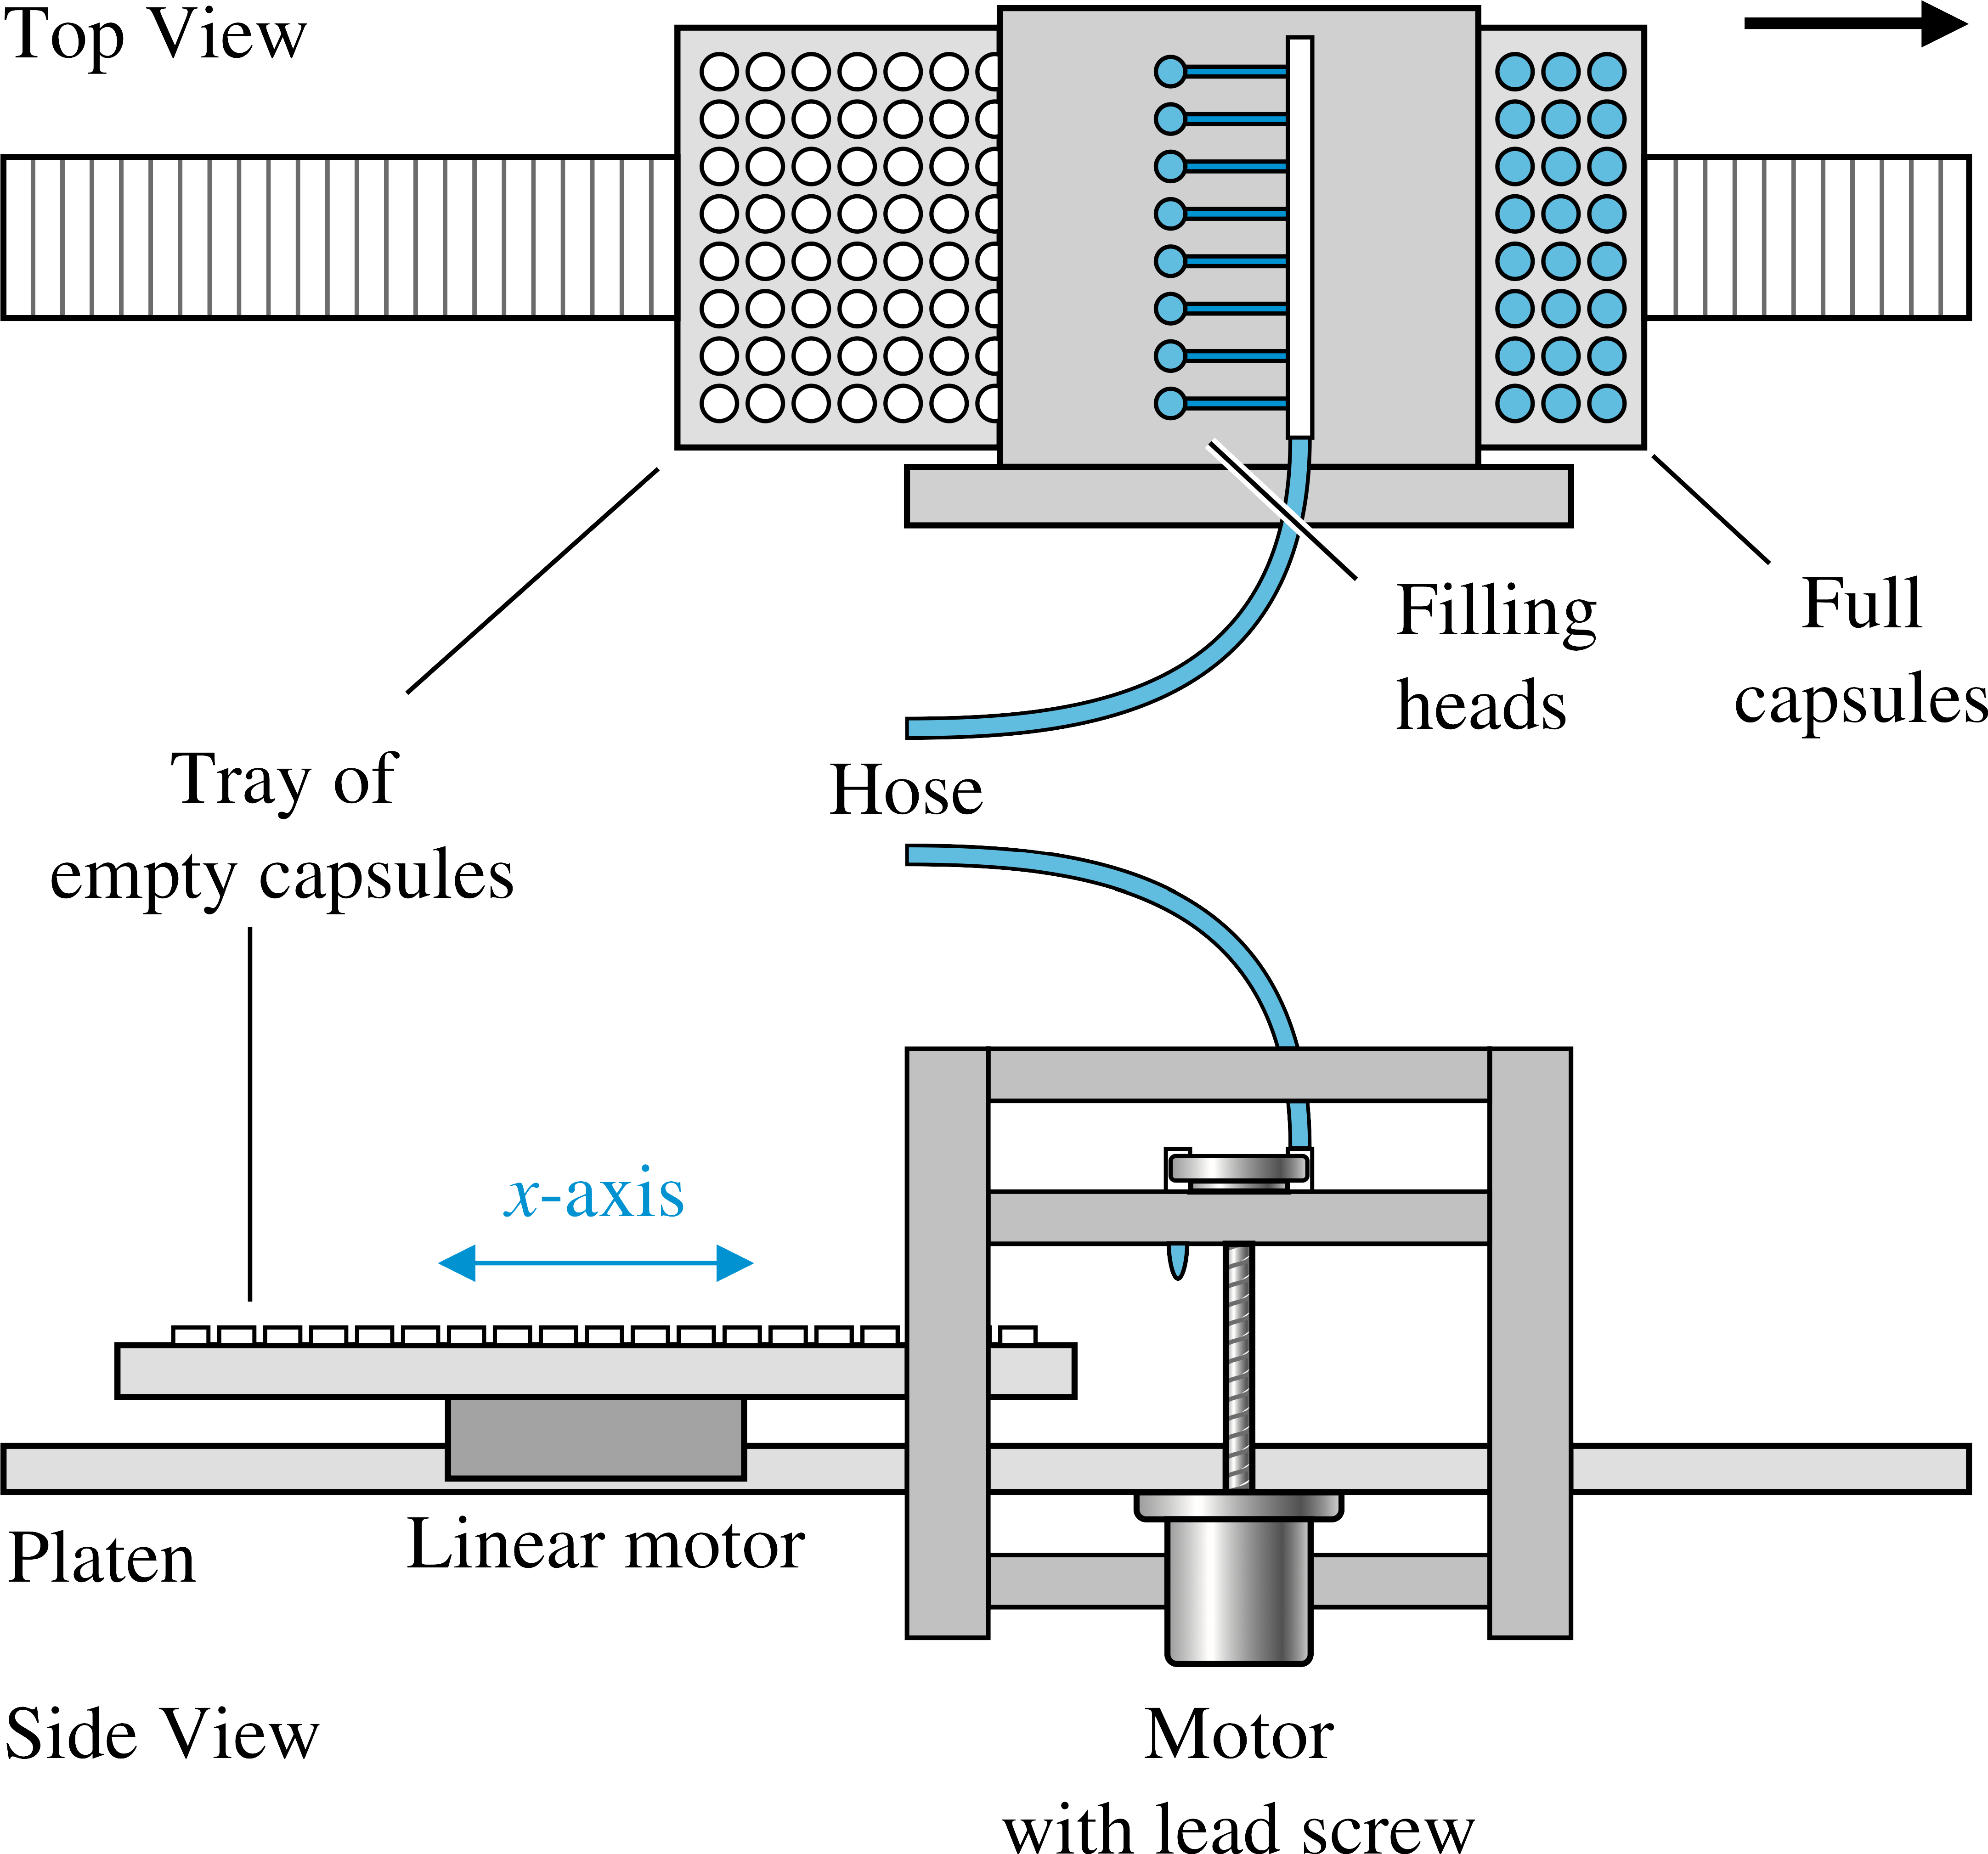
\includegraphics[width=0.4\textwidth]{PS2-Q3.png}
        % \caption{}
        % \label{fig:Title}
    \end{figure}
    \begin{enumerate}
        \item Find the transfer function \(G_1(s)=C_1{(sI-A_1)}^{-1}B_1+D_1\) for System 1.
        \begin{align*}
            G_1(s)&=-\frac{2}{s+2}+\frac{3}{s+3}\\[0.75em]
            &=\frac{s}{s^2+5s+6}
        \end{align*}
        \item Find the transfer function \(G_2(s)=C_2{(sI-A_2)}^{-1}B_2+D_2\) for System 2.
        \begin{align*}
            G_1(s)=\frac{s}{s^2+5s+6}
        \end{align*}
        \item Describe the relationship between \(G_1\) and \(G2\).  What zeros and/or poles do they have in common?\\[1em]
        Even though the state-space representations are different, \(G_1\) and \(G_2\) have the exact same transfer functions. This is because, as the problem stated, state-space representations are not unique and a single system can be represented in several possible ways.
        \begin{align*}
            \text{poles for both: }s&=-2,-3\\
            \text{zeros for both: }s&=0
        \end{align*}
    \end{enumerate}
    \item (+15  points) Consider the following state-space system, that describes the dynamics of a system for automatically dispensing fluid into capsules. A tray of capsules is guided through the dispenser by a linear motor with motor torque \(u(t)\) (the input). The tray position is the output, \(y(t)\).
    \begin{align}
        G(s)=\frac{3}{s^2+Ks+3}
    \end{align}
    \begin{enumerate}
        \item Using Matlab, follow the steps below for each of \(K= 1,2,3,4\). Use the \texttt{diary} or \texttt{publish} commands to record your code, and hand in the history of Matlab command-line inputs and outputs as well as the \textit{single} plot that you generate. \textit{Note: Please append the Matlab file and plot to your homework, so that you hand in a \textbf{single}.pdf. Multiple files will not be accepted.}
        \begin{enumerate}
            \item First create transfer functions \(G_1(s)\text{,} \cdots\text{, } G_4(s)\). For example, for the first system,
\begin{verbatim}
    >> G1 = tf(3, [1 1 3];
\end{verbatim}
            \item On a single figure, plot step responses for each of these systems using
\begin{verbatim}
    >> step(G1,G2,G3,G4)
    >> legend(’G1’,’G2’,’G3’,’G4’)
\end{verbatim}
        Please see the final two pages for Matlab code and figure.
        \end{enumerate}
        \item Consider the oscillatory nature of the step responses. What happens as \(K\) increases? Which value of \(K\) produces the most oscillatory response? Which produces the least?\\[1em]
        \(K\) has the effect of being a dampening agent in our step responses. As \(K\) increases, the oscillations decrease; thus, \(K=1\) is the least damped and most oscillatory response, while \(K=4\) is the most damped and exhibits the least oscillatory response.
    \end{enumerate}
\end{enumerate}
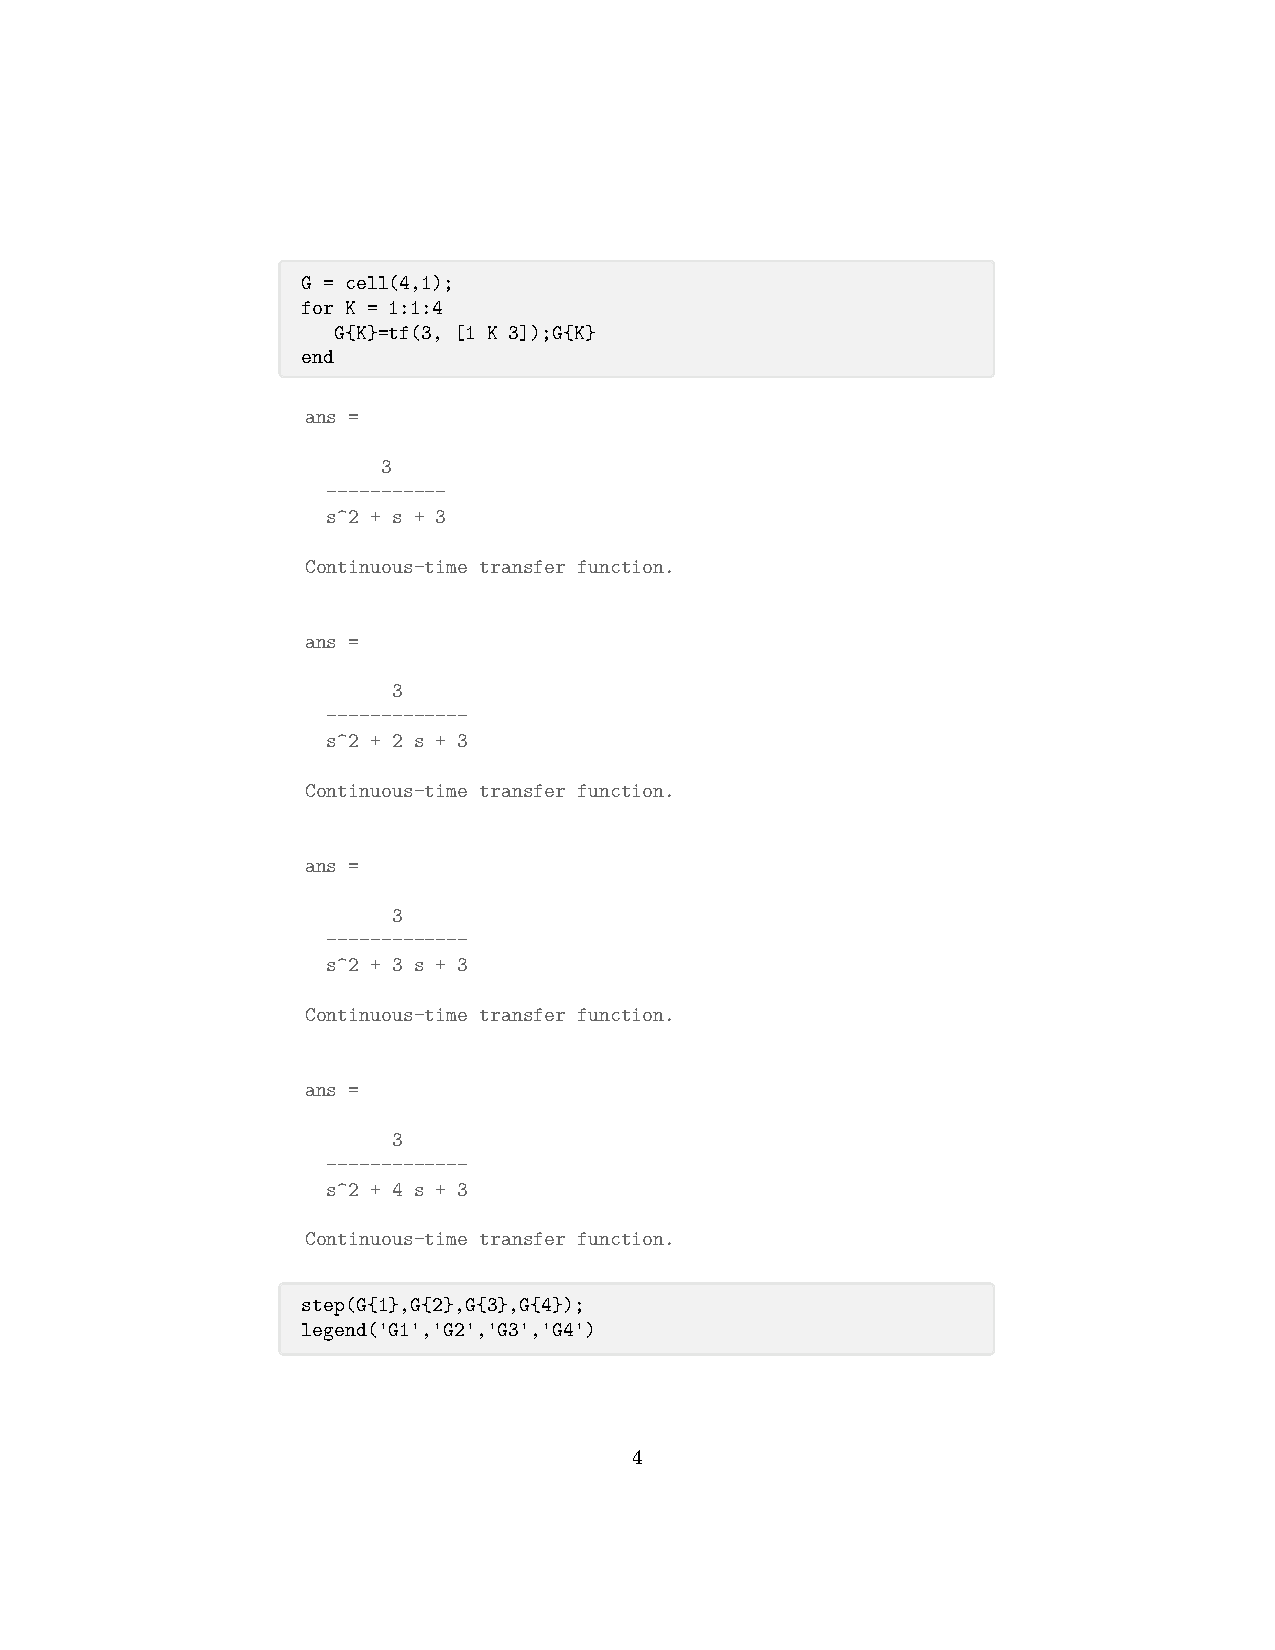
\includepdf[pages=-]{PS02-Matlab.pdf}
\end{document}